\documentclass[12pt,]{article}
\usepackage[T1]{fontenc}
\usepackage{lmodern}
\usepackage{amssymb,amsmath}
\usepackage{ifxetex,ifluatex}
\usepackage{fixltx2e} % provides \textsubscript
% use upquote if available, for straight quotes in verbatim environments
\IfFileExists{upquote.sty}{\usepackage{upquote}}{}
\ifnum 0\ifxetex 1\fi\ifluatex 1\fi=0 % if pdftex
  \usepackage[utf8]{inputenc}
\else % if luatex or xelatex
  \ifxetex
    \usepackage{mathspec}
    \usepackage{xltxtra,xunicode}
  \else
    \usepackage{fontspec}
  \fi
  \defaultfontfeatures{Mapping=tex-text,Scale=MatchLowercase}
  \newcommand{\euro}{€}
    \setmainfont{times}
\fi
% use microtype if available
\IfFileExists{microtype.sty}{\usepackage{microtype}}{}
\usepackage[margin=1in]{geometry}
\usepackage{graphicx}
% Redefine \includegraphics so that, unless explicit options are
% given, the image width will not exceed the width of the page.
% Images get their normal width if they fit onto the page, but
% are scaled down if they would overflow the margins.
\makeatletter
\def\ScaleIfNeeded{%
  \ifdim\Gin@nat@width>\linewidth
    \linewidth
  \else
    \Gin@nat@width
  \fi
}
\makeatother
\let\Oldincludegraphics\includegraphics
{%
 \catcode`\@=11\relax%
 \gdef\includegraphics{\@ifnextchar[{\Oldincludegraphics}{\Oldincludegraphics[width=\ScaleIfNeeded]}}%
}%
\ifxetex
  \usepackage[setpagesize=false, % page size defined by xetex
              unicode=false, % unicode breaks when used with xetex
              xetex]{hyperref}
\else
  \usepackage[unicode=true]{hyperref}
\fi
\hypersetup{breaklinks=true,
            bookmarks=true,
            pdfauthor={},
            pdftitle={},
            colorlinks=true,
            citecolor=blue,
            urlcolor=blue,
            linkcolor=magenta,
            pdfborder={0 0 0}}
\urlstyle{same}  % don't use monospace font for urls
\setlength{\parindent}{0pt}
\setlength{\parskip}{6pt plus 2pt minus 1pt}
\setlength{\emergencystretch}{3em}  % prevent overfull lines
\setcounter{secnumdepth}{0}

\author{}
\date{}
\usepackage{lineno}
\linenumbers
\usepackage{setspace}
\doublespacing

\begin{document}

\normalsize


\section{Microscale models outperform mesoscale models when forecasting
climate change impacts on plant
populations}\label{microscale-models-outperform-mesoscale-models-when-forecasting-climate-change-impacts-on-plant-populations}

\subsubsection[Andrew T. Tredennick and Peter B. Adler]{Andrew T.
Tredennick\footnote{Corresponding author:
  \href{mailto:atredenn@gmail.com}{\href{mailto:atredenn@gmail.com}{atredenn@gmail.com}}}
and Peter B.
Adler}\label{andrew-t.-tredennickcorrauth-and-peter-b.-adler}

\emph{Andrew T. Tredennick, Department of Wildland Resources and the
Ecology Center, Utah State University, Logan, UT}

\emph{Peter B. Adler, Department of Wildland Resources and the Ecology
Center, Utah State University, Logan, UT}

\subsection{Abstract}\label{abstract}

The ability of population models to skillfully forecast future states
under climate change is constrained by the limited spatial and temporal
extent of demographic data. This data is often limited because it is
difficult and costly to collect. An alternative is to rely on aggregate,
population-level data that is easier and less costly to collect. Doing
so requires assuming that population-level data accurately represents
the aggregate response of the individuals that actually respond to
weather. We tested this assumption using population models of four
Montana grassland species fit using individual and aggregated forms of
the same data. We fit population models with interannual variation in
vital rates explained, in part, by climate covariates and then perturbed
observed climate to compare model forecasts. Population models based on
individual-level demographic data outperformed the models based on
aggregate-level data in terms of accuracy and precision. The two model
types produced inconsistent forecasts when we perturbed climate. Thus,
it seems that, at least for the species in this location, demographic
data is necessary to pick up key climate drivers of vital rates like
survival that are not well resolved in aggregated data. On a pessimistic
note, our work shows that even with detailed demographic data, model
forecasts are extremely uncertain. It is becoming clear the long time
series (over two decades) are necessary to produce meaningful forecasts.

\emph{Keywords}: forecasting, climate change, grassland, integral
projection model, population model

\subsection{Introduction}\label{introduction}

Population models are important tools for predicting the impacts of
environmental change on species. But reconciling the scales at which
population models are parameterized and the scales at which
environmental changes play out remains a challenge (Clark et al. 2010,
2012, Freckleton et al. 2011, Queenborough et al. 2011). The major
hurdle is that most population models, at least for plant species, are
built using data from small, localized plots because parameterizing
traditional population models requires tracking the fates of
individuals. These models are difficult to scale up from the micro to
meso-scales because the fitted parameters do not fully represent the
spatial variation present at scales beyond that at which the data are
collected (Sæther et al. 2007). At the same time, most demographic data
is collected over short time spans. For example, the most common study
duration in the COMPADRE matrix population model database is 4 years and
only a few exceed 10 years (Salguero-Gómez et al. 2015). The constrained
spatio-temporal extent of most demographic datasets reflects the
difficulty of collecting such data, but those constraints limit our
ability to extrapolate population models. Thus, our ability to use
population models to predict the consequences of climate change is
limited when we rely on individual-level data.

Aggregate measures of individual plant performance, such as those
typically collected as part of large-scale census efforts, offer an
alternative to detailed demographic data for modeling populations (Clark
and Bjørnstad 2004, Freckleton et al. 2011). Such population-level data
will never match the precision of individual-level data, but it is more
feasible to attain a broad coverage sample when collecting coarse-scale
data. This presents a difficult trade-off: on the one hand,
individual-level data leads to more reliable models; on the other hand,
population-level data leads to models that will produce less precise
predictions but can be applied over greater spatial and temporal
extents. An open question is how well models based on population-level
data compare to models based on individual-level data.

To date, relatively few studies have tried to model populations based on
data other than detailed individual-level data. An important exception
is an effort by Taylor and Hastings (2004) to model the population
growth rate of an invasive species to investigate the best strategies
for invasion control. They used a ``density-structured'' model where the
state variable is a discrete density state rather than a continuous
density measure. Building on this work, Freckleton et al. (2011) showed
that density-structured models compare well to continuous models in
theory, and Queenborough et al. (2011) showed the application of such
methods in a study on arable weeds. In particular, Queenborough et al.
(2011) provide empirical evidence that density-structured models are
capable of reproducing population dynamics, even if some precision is
lost when compared to fully continuous models. Thus, population models
based on coarse, population-level data show promise for producing
ecological forecasts at landscape and regional scales (Queenborough et
al. 2011). However, none of these models included environmental
covariates.

Basing population models on aggregated individual-level data in a
climate change context is hampered by the fact that it is individuals
that respond to climate, not populations (Clark et al. 2012). This fact
puts us in uneasy proximity to an ``ecological fallacy'' where one
deduces inference on the individual from statistical inference on the
group (Piantadosi et al. 1988). For example, individual plants may
respond positively to precipitation but a negative trend is observed at
the population level due to increased competition among plants as they
grow larger and consume more resources. Thus, it is important to ask the
question: Can aggregated data be used to detect climate signals of the
same sign and magnitude as individual-level data? If not, then building
population models with climate covariates on aggregated data will lead
to incorrect forecasts.

Here, we test the assumption that statistical and population models
based on aggregated data can detect climate signals as wells as models
based on individual-level data. We use a unique demographic dataset that
tracks the fates of individual plants from four species over 14 years to
build single-species population models, since those are often used tools
for ecological forecasts and climate vulnerability assessments. We first
fit population models with interannual variation in vital rates
explained, in part, by climate covariates. We then perturb the climate
covariates to test the sensitivities of species to climate change. By
doing these analyses using both individual and aggregated forms of the
same data we can directly compare the two types of models.

In general, we find that population models based on detailed demographic
data are more accurate and precise than models based on aggregated data.
Both types of models are able to detect climate signals, as evidenced by
the sensitivity of simulated equilbrium plant cover under a perturbed
climate scenario. But the two types of models produce inconsistent
forecasts, in some cases producing completely opposing predictions. This
leads us to conclude that, at least for these species at this location,
detailed demographic data is necessary to detect the ``right'' climate
signal. A worrying caveat to our work is that forecasts from both models
were very uncertain. It seems that even 14 years worth of demographic
data is not enough to produce meaningful forecasts when model
uncertainty is explicitly considered.

\subsection{Materials and Methods}\label{materials-and-methods}

\subsubsection{Study site and data}\label{study-site-and-data}

Our demographic data comes from the Fort Keogh Livestock and Range
Research Laboratory in eastern Montana's northern mixed prairie near
Miles City, Montana, USA ($46^{\circ}$ 19' N, $105^{\circ}$ 48' W). The
dataset is freely available on Ecological Archives\footnote{\url{http://esapubs.org/archive/ecol/E092/143/}}
(Anderson et al. 2011) , and interested readers should refer to the
metadata therein for a complete description. The site is about 800 m
above sea level and mean annual precipitation (1878-2009) is 334 mm,
with most annual precipitation falling from April through September. The
site is grass dominated and, for the purposes of our study, we focus on
the four most abundant graminoid species: \emph{Bouteloua gracilis}
(BOGR), \emph{Hesperostipa comata} (HECO), \emph{Pascopyrum smithii}
(PASM), and \emph{Poa secunda} (POSE).

From 1932 to 1945 individual plants were identified and mapped annually
in 44 1-$\text{m}^2$ quadrats using a pantograph. The quadrats were
distributed in six pastures, each assigned a grazing treatment of light
(1.24 ha/animal unit month), moderate (0.92 ha/aum), and heavy (0.76
ha/aum) stocking rates (two pastures per treatment). In this analysis we
account for potential differences among the grazing treatments, but do
not focus on grazing$\times$climate interactions. The annual maps of the
quadrats were digitized and the fates of individual plants tracked and
extracted using a computer program. Daily climate data, which we
aggregated into climate variables of interest, are available for the
duration of the data collection period (1932 - 1945) from the Miles City
airport, Wiley Field, 9 km from the study site.

In this paper, we model populations based on two levels of data:
individual and quadrat (Fig. 1). The individual data is the ``raw''
data. For the quadrat level we data we simply sum individual areal cover
for each quadrat by species. This is equivalent to a perfect census of
quadrat percent cover, so we do not need to consider measurement error.
Based on these two datasets we can compare population models built using
individual level data and aggregated quadrat level data.

All R code and data necessary to reproduce our analysis is archived on
GitHub as release 1.0
(\url{http://github.com/atredennick/MicroMesoForecast/releases}). That
stable release will remain static as a record of this analysis, but
subsequent versions may appear if we update this work.

\subsubsection{Stastical models of vital
rates}\label{stastical-models-of-vital-rates}

At both levels of inference (individual and quadrat), the building
blocks of our population models are vital rate regressions. For
individual level data we fit models for survival, growth, and
recruitment of new individuals for each species. At the quadrat level we
fit a single regression model for population growth. We describe the
statistical models separately since fitting the models required
different approaches. All models contain five climate covariate that we
chose \emph{a priori}: ``water year'' precipitation at \emph{t}-1
(lagppt); fall through spring precipitation at \emph{t}-1 and \emph{t}-2
(ppt1 and ppt2, respectively) and mean spring temperature at \emph{t}-1
and \emph{t}-2 (TmeanSpr1 and TmeanSpr2, respectively), where \emph{t}
is the observation year. We also include interactions among same-year
climate covariates (e.g., ppt1 $\times$ TmeansSpr1) and climate $\times$
size interactions.

We fit all models using a hierarchical Bayesian approach, which we
describe in more detail below. However, for each vital rate statistical
model we also define the likelihood model we use. For the likelihood
models, \textbf{Y} is always the relevant vector of observations (e.g.,
whether a genet survived {[}1{]} or not {[}0{]} from year $t$ to $t+1$).

\paragraph{Vital rate models at the individual
level}\label{vital-rate-models-at-the-individual-level}

We used logistic regression to model survival probability ($S$) of genet
$i$ from species $j$ in quadrat group $Q$ from time $t$ to $t+1$:

\begin{align}
\text{logit}(S_{ijQ,t}) &= \gamma^{S}_{j,t} + \phi^{S}_{jQ} + \beta^{S}_{j,t}x_{ij,t} + \omega^{S}_{j}w_{ij,t} + \theta^{S}_{jk}C_{k,t} + \varepsilon^{S}_{t} \\
Y^{S}_{ijQ,t} &\sim \text{Bernoulli}(S_{ijQ,t})
\end{align}

where $x_{ij,t}$ is the log of genet size, $\gamma^{S}_{j,t}$ is a
year-specific intercept, $\beta^{S}_{j,t}$ is the year-specific slope
parameter for size, $\phi^{S}_{jQ}$ is the random effect of quadrat
group location, and $\theta^{S}_{k}$ is the fixed parameter for the
effect of the $k$th climate covariate at time $t$ ($C_{k,t}$). We
include density-dependence by estimating the effect of crowding on the
focal individual by other individuals of the same species. $\omega$ is
the effect of crowding and $w_{t,Q}$ is the crowding experienced by the
focal individual at time $t$ in quadrat group $Q$.

We modeled growth as Gaussian process describing genet size at time
$t+1$ as a function of size at $t$ and climate covariates:

\begin{align}
x_{ijQ,t+1} &= \gamma^{G}_{j,t} + \phi^{G}_{jQ} + \beta^{G}_{j,t}x_{ij,t} + \omega^{G}_{j}w_{ij,t} + \theta^{G}_{jk}C_{k,t} \\
Y^{G}_{ijQ,t} &\sim \text{Normal}(x_{ijQ,t+1}, \sigma_{j})
\end{align}

where $x$ is log genet size and all other parameters are as described
for the survival regression.

Our data allows us to track new recruits, but we cannot assign a
specific parent to new genets. So, for recruitment, we work at the
quadrat level and model the number of new individuals of species $j$ in
quadrat $q$ recruiting at time $t+1$ as a function of quadrat
``effective cover'' ($A'$) in the previous year ($t$). Effective cover
is a mixture of observed cover ($A$) in the focal quadrat ($q$) and the
mean cover across the entire group ($\bar{A}$) of $Q$ quadrats in which
$q$ is located:

\begin{equation}
A'_{jq,t} = p_{j}A_{jq,t} + (1-p_{j})\bar{A}_{jQ,t}
\end{equation}

where $p$ is a mixing fraction between 0 and 1 that is estimated within
the model.

We assume the number of individuals, $Y^{R}$, recruiting at time $t+1$
follows a negative binomial distribution:

\begin{equation}
Y^{R}_{jq,t+1} \sim \text{NegBin}(\lambda_{jq,t+1},\zeta)
\end{equation}

where $\lambda$ is the mean intensity and $\zeta$ is the size parameter.
We define $\lambda$ as:

\begin{equation}
\lambda_{jq,t+1} = A'_{jq,t}e^{(\gamma^{R}_{j,t} + \phi^{R}_{jQ} + \theta^{R}_{jk}C_{k,t} + \omega^{R}\sqrt{A'_{q,t}})}
\end{equation}

where $A'$ is effective cover ($\text{cm}^2$) of species $j$ in quadrat
$q$ and all other terms are as in the survival and growth regressions.

\paragraph{Population model at the quadrat
level}\label{population-model-at-the-quadrat-level}

The statistical approach used to model vital rates using aggregated data
depends on the type of data collected. In our case, and as is often the
case with census data, we have percent cover data (which can easily be
transformed to proportion data, of course). We first considered fitting
three vital rate models analagous to those we fit at the individual
level: one for probability of extirpation within a quadrat (analagous to
survival), one for cover change within a quadrat (analagous to growth),
and one for probability of colonization within a quadrat (analagous to
recruitment). However, within-quadrat extirpation and colonization
events were rare in our time series ($N=9$ and $N=10$, respectively
across all species). Given the broad spatial distribution of the
quadrats we are studying, it is safe to assume that these events are in
fact rare enough to be ignored for our purposes. So we constrained our
statistical modeling of vital rates at the population level to change in
percent cover within quadrats. For the remaining discussion of
statistical modeling we refer to proportion data, which is simply
percent data divided by 100.

An obvious choice for fitting a linear model to proportion data is beta
regression because the support of the beta distribution is {[}0,1{]},
not including true zeros or ones. However, when we used fitted model
parameters from a beta regression in a quadrat-based population model
the simulated population tended toward 100\% cover for all species. We
therefore chose a more constrained modeling approach based on a
truncated log-normal likelihood. The model for quadrat cover change
($G$) from time $t$ to $t+1$ is

\begin{align}
x_{jq,t+1} &= \gamma^{G}_{j,t} + \phi^{G}_{jQ} + \beta^{G}_{j,t}x_{jq,t} + \theta^{S}_{jk}C_{k,t} \\
Y^{G}_{jq,t+1} &\sim \text{LogNormal}(x_{jq,t+1}, \tau{j}) \text{T}[0,1]
\end{align}

where $x_{jq,t}$ is the log of species' $j$ proportional cover in
quadrat $q$ at time $t$ and all other parameters are as in the
individual-level growth model (Eq. \#). The log normal likelihood
includes a truncation (T{[}0,1{]}) to ensure that predicted values do
not exceed 100\% cover.

\subsubsection{Model fitting}\label{model-fitting}

Our Bayesian approach to fitting the vital rate models required choosing
appropriate priors for unknown parameters and deciding which, if any, of
those priors should be hierarchical. We decided to fit models where all
terms were fit by species. Within a species, we fit yearly size effects
and yearly intercepts hierarchically where year-specific coefficients
were drawn from global distributions representing the mean size effect
and intercept. We used flat, uninformative priors for all unknown
parameters (Appendix X).

All of our analyses (model fitting and simulating) were conducted in R
(R Core Development Team 2013). We used the `No-U-Turn' MCMC sampler in
Stan (Stan Development Team 2014a) to estimate the posterior
distributions of model parameters using the package `rstan' (Stan
Development Team 2014b). We obtained posterior distributions for all
model parameters from three parallel MCMC chains run for 1,000
iterations after discarding an initial 1,000 iterations. We recignize
such short MCMC chains may surprise those more familiar with other MCMC
samplers (i.e.~JAGS or WinBUGS), but the Stan sampler is exceptionally
efficient, which reduces the number of iterations needed to achieve
convergence. We assessed convergence visually and made sure scale
reduction factors for all parameters were less than 1.01. For the
purposes of including parameter uncertainty in our population models, we
saved the final 1,000 iterations from each of the three MCMC chains for
all parameters to be used as randomly drawn values during population
simulation. This step alleviates the need to reduce model parameters by
model selection since sampling from the full parameter space in the MCMC
ensures that if a parameter broadly overlaps zero, on average the effect
in the population models will also be near zero.

\subsubsection{Population models}\label{population-models}

With the posterior distribution of the vital rate statistical models in
hand, it is straightforward to simulate the population models. We used
an Integral Projection Model (IPM) to model populations based on
individual level data and an quadrat based version of an
individually-based model (Quadrat-Based Model, QBM) to model populations
based on quadrat level data. We describe each in turn.

\paragraph{Integral projection model}\label{integral-projection-model}

We use an environmentally stochastic IPM (Rees and Ellner 2009) that
includes the random year effects and the climate covariates from the
vital rate statistical models. But note that we can, and do for some
simulations, ignore the random year effects so that only the climate
effects can drive interannual variation. Our IPM follows the
specification of Chu and Adler (2015) where the population of species
\emph{j} is a density function $n(u_{j},t)$ giving the density of
sized-\emph{u} genets at time \emph{t}. Genet size is on the natural log
scale, so that $n(u_{j},t)du$ is the number of genets whose area (on the
arithmetic scale) is between $e^{u_{j}}$ and $e^{u_{j}+du}$. So, the
density function for any size \emph{v} at time $t+1$ is

\begin{equation}
n(v_{j},t+1) = \int_{L_{j}}^{U_{j}} k_{j}(v_{j},u_{j},\bar{\bold{w_{j}}}(u_{j}))n(u_{j},t)
\end{equation}

where $k_{j}(v_{j},u_{j},\bar{\bold{w_{j}}})$ is the population kernal
that describes all possible transitions from size $u$ to $v$ and
$\bar{\bold{w_{j}}}$ is a vector of estimates of average crowding
experienced from all other species by a genet of size $u_j$ and species
$j$. The integral is evaluated over all possible sizes between
predefined lower (\emph{L}) and upper (\emph{U}) size limits that extend
beyond the range of observed genet sizes.

The population kernal is defined as the joint contributions of survival
(\emph{S}), growth (\emph{G}), and recruitment (\emph{R}):

\begin{equation}
k_{j}(v_{j},u_{j},\bar{\bold{w_{j}}}) = S_j(u_j, \bar{\bold{w_{j}}}(u_{j}))G_j(v_{j},u_{j},\bar{\bold{w_{j}}}(u_{j})) + R_j(v_{j},u_{j},\bar{\bold{w_{j}}}),
\end{equation}

which, said plainly, means we are calculating growth (\emph{G}) for
individuals that survive (\emph{S}) from time \emph{t} to \emph{t+1} and
adding in newly recruited (\emph{R}) individuals of an average sized
one-year-old genet for the focal species. Our stastical model for
recruitment (\emph{R}, described above) returns the number of new
recruit produced per quadrat. Following previous work (Adler et al.
2012, Chu and Adler 2015), we assume that fecundity increases linearly
with size
($R_j(v_{j},u_{j},\bar{\bold{w_{j}}}) = e^{u_j}R_j(v_{j},\bar{\bold{w_{j}}})$)
to incorporate the recruitment function in the spatially-implicit IPM.

We used random draws from the final 1,000 iterations from each of three
MCMC chains to introduce stochasticity into our population models. At
each time step, we randomly selected climate covariates from one of the
14 observed years. Then, we drew the full parameter set (climate effects
and density-dependence fixed effects) from a randomly selected MCMC
iteration. Using this approach, rather than simply using coefficient
point estimates, ensures that relatively unimportant climate covariates
(those that broadly overlap 0) have little effect on the simulation
results. Since our focus was on the contribution of climate covariates
to population states, we set the random year effects and the random
group effects to zero.

\paragraph{Quad-based model}\label{quad-based-model}

Our quad-based model (QBM) perfectly mirrors its statistical description
(Eq. \#). We use the same approach for drawing parameter values as
described for the IPM.

\subsubsection{Model validation}\label{model-validation}

To test each model's ability to forecast the population state we made
out of sample predictions using leave-one-year-out cross validation. For
both levels of modeling, we fit the vital rate models using observations
from all years except one, and then used those fitted parameters in the
population models to perform a one-step-ahead forecast for the year
whose observations were withheld from model fitting. Within each
observation year, several quadrats are sampled. So we made predictions
for each observed quadrat in the focal year initialized with cover the
previous year. Since we were making quadrat specific predictions we
incorporated the group effect on the intercept for both models. We
repeated this procedure for all 13 observation years, making 100
one-step-ahead forecasts for each quadrat-year combination with
parameter uncertainty included via randomdrawd from the MCMC chain as
described above. Random year effects were set to zero since year effects
cannot be assigned to unobserved years.

This model validation allowed us to compare accuracy and precision of
the two modeling approaches (individual-level versus population-level).
We first calculated the median predicted cover across the 100
simulations for each quadrat-year and then calculated the absolute error
as the difference between the observed cover for a given quadrat-year
and the median prediction. To arrive at mean absolute error (MAE), we
then averaged the absolute error within each species across the
quadrat-year specific errors. We use MAE as our measure of accuracy. To
measure precision we calculated the distance between the upper and lower
90th quantiles of the 100 predictions and averaged this value over
quadrat-years for each species.

\subsubsection{Testing sensitivity to climate
covariates}\label{testing-sensitivity-to-climate-covariates}

Our main goal in this paper is to see if models based on aggregate level
data are as sensitive to climate as models based on individual level
data. So, with our fitted and validated models in hand, we ran
simulations for each model type (IPM and QBM) under four climate
perturbation scenarios: (1) observed climate, (2) precipitation
increased by 1\%, (3) temperature increased by 1\%, and (4)
precipitation and temperature increased by 1\%. We ran the simulations
for 2,500 time steps, enough to estimate equilibrium cover after
discarding an initial 500 time steps as burn-in. Each simulation was run
under two parameter scenarios: (1) using mean parameter estimates and
(2) using randomly drawn parameters from the MCMC chain. We use (1) to
detect the overall sensitivity of equilibrium cover to climate, and we
use (2) to show the impact of model uncertainty on forecast precision.

As an effort to identify potential discrepencies between IPM and QBM
forecasts, we also ran simulations designed to quantify the
sensitivities of individual and combined vital rates to climate for the
IPM. Specifically, we ran simulations for the above climate scenarios,
but applied the perturbed climate covariates to survival, growth, and
recruitment vital rates individually and in pairwise combinations. This
allows us to isolate the vital rate(s) most sensitive to climate. For
this analysis, we used mean parameter estimates to reduce the sources of
uncertainty in the sensitivity estimates.

\subsection{Results}\label{results}

\subsubsection{Comparison of forecast
models}\label{comparison-of-forecast-models}

The IPM had significantly lower overall error (MAE, mean absolute error)
for three species (\emph{B. gracilis}, \emph{H. comata}, \emph{P.
smithii}; Table 1). In no case did the QBM significantly outperform the
IPM (Table 1). The IPM was consistently more precise than the QBM, with
lower distances between the 90\% quantiles across all species (Table 1).
In general the IPM outperformed the QBM because it had (1) lower MAE for
three of the four species, (2) statistically similar MAE for the one
other species, and (3) considerably more precise forecasts for all
species.

\subsubsection{Sensitivity of models to
climate}\label{sensitivity-of-models-to-climate}

Equilibrium cover from both models was sensitive to climate (Fig. 2a-d).
The IPM projected percent changes in equilibrium cover from -3 - 8\% for
\emph{B. gracilis}, -4 - 3\% for \emph{H. comata}, -15 - 9\% for
\emph{P. smithii}, and -17 - 53\% for \emph{P. secunda}. The QBM
projected opposite and greater percent changes in equilibrium cover for
\emph{B. gracilis} (-63 - 30\%) and \emph{H. comata} (-50 - -18\%; Fig.
2a-b). For \emph{P. smithii}, the QBM projected opposite changes in
equilibrium cover than the IPM, but of similar magnitude (-5 - 6\%; Fig.
2C). \emph{P. secunda} was the only species that the IPM and QBM made
projections of the same sign and somewhat similar magnitude (Fig. 2d).
As expected based on model validation (Table 1), IPM projections were
more uncertain than QBM projections for all species and all climate
change scenarios (Fig. 2e-h).

The response of a population to climate change is a result of the
aggregate effects of climate on individual vital rates. Since the IPM
approach relies on vital rate regressions, we were able to quantify the
sensitivity of each vital rate in isolation and in pairwise
combinations. Species showed similar trends (Fig. 3). Growth was the
most sensitive vital rate for all species, showing a negative response
to increased precipitation, and stronger positive response to increased
temperature, and a mostly positive response when both climate factors
are increased (Fig. 3). \emph{B. gracilis} survival rates were sensitive
to temperature, resulting in an increase in plant cover under increased
temperature (Fig. 3a). In isolation, recruitment and survival were
insensitive to climate factors for \emph{H. comata} (Fig. 3b). Survival
and recruitment of \emph{P. smithii} were both sensitive, negatively, to
temperature and precipitation (Fig. 3c). \emph{P. secunda} equilibrium
cover was sensitive to the climate effects on survival and recruitment,
showing a negative effect on both vital rates for increased precipition,
but a strong positive effect on survival with increased temperature
(Fig. 3d). The climate impact of recruitment on equilibrium cover was
negative for precipitation and temperature increases (Fig. 3d).

\subsection{Discussion}\label{discussion}

Demographic models are costly to parameterize, yet remain the most
widely-used tools for studying plant population dynamics (e.g.,
Salguero-Gómez et al. (2015)). New density-structured approaches
sacrifice some precision at the local scale for better spatial coverage
that is virtually unattainable, due to time and funding constraints,
using traditional individual-based data (Freckleton et al. 2011,
Queenborough et al. 2011). These approaches are appealing because
traditional population models suffer from constrained parameter space --
meaning forecasts quickly extend beyond the parameter space used to fit
the model. Density-structured approaches rely on easy-to-collect census
data (e.g., percent cover in $1\text{m}^2$ quadrats) so sampling
populations across large spatial extents would be possible, thus
covering more potential parameter space.

Estimating parameter variability in space and time is critical when
using population models to forecast responses to directional changes in
exogoneous drivers like climate ({\textbf{???}}, {\textbf{???}},
{\textbf{???}}, {\textbf{???}}). Compared to demographic models,
density-structured modeling approaches may provide an efficient route
toward estimating such uncertainty. However, population models based on
aggregated inidividual data have yet to be tested with climate drivers.
Since it is individuals that respond to weather, rather than
populations, models based on a aggregated data may produce incorrect
forecasts (Clark et al. 2012). Thus, we sought to compare climate
sensitivities of individual and population based models of four
grassland species populations.

\subsubsection{Forecasting the future, and the future of
forecasting}\label{forecasting-the-future-and-the-future-of-forecasting}

Our goal was not make any explicit forecast for the future state of
these populations based on predicted climate change. But our results
highlight the state of affairs in ecology when it comes to forecasting
the impacts of climate change. The analysis we conducted here could be
considered, with some exceptions of course, at the forefront of
ecological forecasting in terms of the statistical approach employed
(hierarchical Bayesian), the type of population model we used
(stochastic IPM with parameter uncertainty), and the amount of data we
had at our disposal (14 years of individual-level data). Yet, model
predictions proved so uncertain that any forecast, when bounded with
uncertainty, would be at best not useful and at worst meaningless.

Something about fitting the models\ldots{}then cite Britta's paper:
20-25 years needed!

\subsection{Acknowledgments}\label{acknowledgments}

This work was funded by the National Science Foundation through a
Postdoctoral Research Fellowship in Biology to ATT (DBI-1400370) and a
CAREER award to PBA (DEB-1054040). We thank the original mappers of the
permanent quadrats in Montana and the digitizers in the Adler lab,
without whom this work would not have been possible. Informal
conversations with Stephen Ellner, Giles Hooker, Robin Snyder, and a
series of meetings among the Adler and Weecology labs at USU sharpened
our thinking.

\pagebreak{}

\subsection{Tables}\label{tables}

\begin{table}[ht]
\centering
\caption{Accuracy (mean absolute error, MAE) and precision (90\% Distance) of out of sample predictions. Forecasts were made without random year effects; only climate covariates could explain year-to-year variation. 90\% Distance refers to the average distance between the upper and lower 90th percentiles of the 100 predicted values for each quadrat-year combination.} 
\begin{tabular}{llrrr}
  \hline
Species & Model & MAE & 90\% Distance & Mean Obs. Cover \\ 
  \hline
BOGR & IPM & 12.18 & 38.52 & 9.43 \\ 
  BOGR & QBM & 19.66 & 56.50 & 9.26 \\ 
  HECO & IPM & 1.22 & 6.47 & 1.15 \\ 
  HECO & QBM & 12.35 & 41.11 & 1.18 \\ 
  PASM & IPM & 0.19 & 1.65 & 0.42 \\ 
  PASM & QBM & 0.55 & 7.78 & 0.42 \\ 
  POSE & IPM & 1.37 & 7.64 & 1.25 \\ 
  POSE & QBM & 1.79 & 40.59 & 1.27 \\ 
   \hline
\end{tabular}
\end{table}

\emph{NOTES}: The IPM MAE is significantly lower at $\alpha=0.05$ for
\emph{B. gracilis} (\emph{P} = 0.0012), \emph{H. comata} (\emph{P} =
4.0586 × 10-8), and \emph{P. smithii} (\emph{P} = 3.183 × 10-5). MAEs
are statisticially similar between models for \emph{P. secunda}
(\emph{P} = 0.0922).

\pagebreak{}

\pagebreak{}

\subsection{Figures}\label{figures}

\begin{figure}[htbp]
\centering
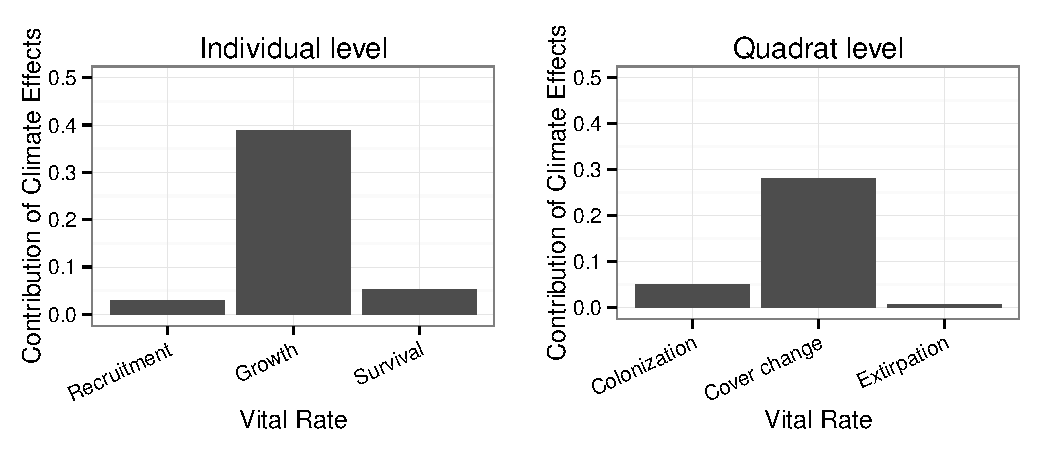
\includegraphics{components/figure/manuscript-figure_1.pdf}
\caption{Work flow of the data aggregation, model fitting, and
population simulating.}
\end{figure}

\begin{figure}[htbp]
\centering
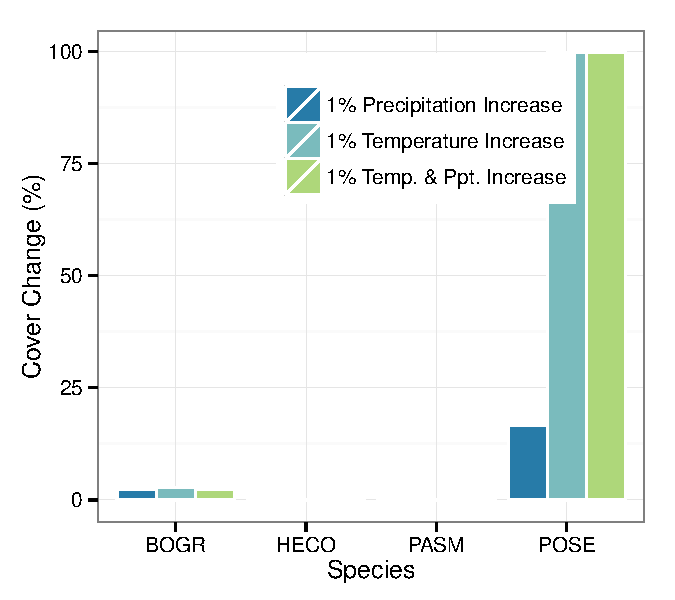
\includegraphics{components/figure/manuscript-figure_2.pdf}
\caption{Proportional change in species' mean cover caused by a 1\%
increase in observed precipitation (+ppt), temperature (+temp), or both
(+ppt\&temp) as predicted by the individual-based IPM and the
aggregate-based QBM. Top panels show the mean predicted proportional
change in cover; lower panels show the 90\% quantiles of predicted
proportional cover change. Mean predictions and their associated
uncertainties are shown in separate panels for visual clarity.}
\end{figure}

\begin{figure}[htbp]
\centering
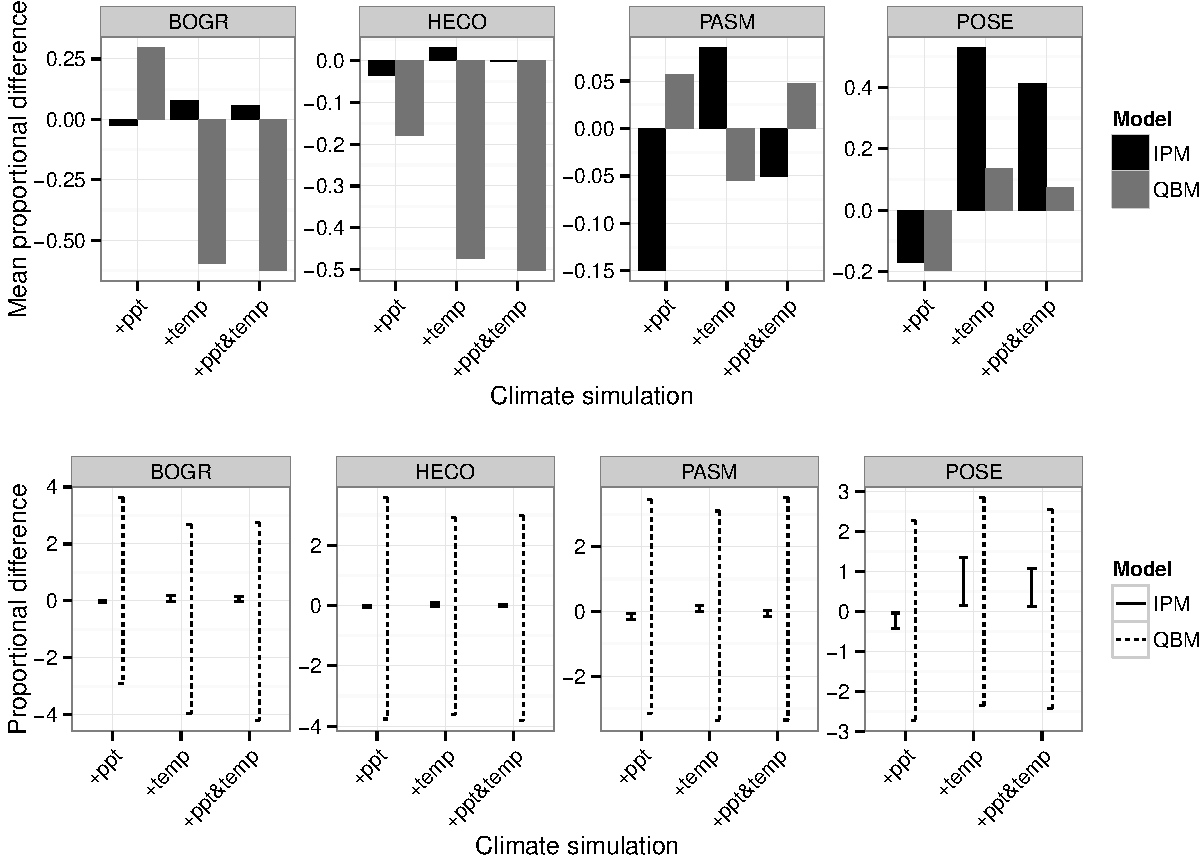
\includegraphics{components/figure/manuscript-figure_3.pdf}
\caption{Sensitivity of equilibrium cover to a 1\% increase in
precipitation (+ppt), temperature (+temp), or both (+ppt\&temp) applied
to individual and combined vital rates. For example, the points
associated with G show the median cover from IPM simulations where a
climate perturbation is applied only to the growth regression climate
covariates.}
\end{figure}

\pagebreak{}

\subsection{References}\label{references}

Adler, P. B., H. J. Dalgleish, and S. P. Ellner. 2012. Forecasting plant
community impacts of climate variability and change: when do competitive
interactions matter? Journal of Ecology 100:478--487.

Anderson, J., L. Vermeire, and P. B. Adler. 2011. Fourteen years of
mapped, permanent quadrats in a northern mixed prairie, USA. Ecology
92:1703.

Chu, C., and P. B. Adler. 2015. Large niche differences emerge at the
recruitment stage to stabilize grassland coexistence. Ecological
Monographs.

Clark, J. S., and O. N. Bjørnstad. 2004. Population time series: Process
variability, observation errors, missing values, lags, and hidden
states. Ecology 85:3140--3150.

Clark, J. S., D. M. Bell, M. Kwit, A. Stine, B. Vierra, and K. Zhu.
2012. Individual-scale inference to anticipate climate-change
vulnerability of biodiversity. Philosophical Transactions of the Royal
Society B: Biological Sciences 367:236--246.

Clark, J. S., D. Bell, C. Chu, B. Courbaud, M. Dietze, M. Hersh, J.
HilleRisLambers, I. Ibáñez, S. LaDeau, S. McMahon, J. Metcalf, J. Mohan,
E. Moran, L. Pangle, S. Pearson, C. Salk, Z. Shen, D. Valle, and P.
Wyckoff. 2010. High-dimensional coexistence based on individual
variation: a synthesis of evidence. Ecological Monographs 80:569--608.

Freckleton, R. P., W. J. Sutherland, A. R. Watkinson, and S. A.
Queenborough. 2011. Density-structured models for plant population
dynamics. American Naturalist 177:1--17.

Piantadosi, S., D. P. Byar, and S. B. Green. 1988. The Ecological
Fallacy. American Journal of Epidemiology 127:893--904.

Queenborough, S. A., K. M. Burnet, W. J. Sutherland, A. R. Watkinson,
and R. P. Freckleton. 2011. From meso- to macroscale population
dynamics: A new density-structured approach. Methods in Ecology and
Evolution 2:289--302.

R Core Development Team. 2013. R: A language and environment for
statistical computing.

Rees, M., and S. P. Ellner. 2009. Integral projection models for
populations in temporally varying environments. Ecological Monographs
79:575--594.

Salguero-Gómez, R., O. R. Jones, C. R. Archer, Y. M. Buckley, J.
Che-Castaldo, H. Caswell, D. Hodgson, A. Scheuerlein, D. A. Conde, E.
Brinks, H. de Buhr, C. Farack, F. Gottschalk, A. Hartmann, A. Henning,
G. Hoppe, G. Römer, J. Runge, T. Ruoff, J. Wille, S. Zeh, R. Davison, D.
Vieregg, A. Baudisch, R. Altwegg, F. Colchero, M. Dong, H. de Kroon,
J.-D. Lebreton, C. J. E. Metcalf, M. M. Neel, I. M. Parker, T. Takada,
T. Valverde, L. A. Vélez-Espino, G. M. Wardle, M. Franco, and J. W.
Vaupel. 2015. The compadrePlant Matrix Database: an open online
repository for plant demography. Journal of Ecology 103:202--218.

Stan Development Team. 2014a. Stan: A C++ Library for Probability and
Sampling, Version 2.5.0.

Stan Development Team. 2014b. Rstan: the R interface to Stan, Version
2.5.0.

Sæther, B. E., S. Engen, V. Grøtan, W. Fiedler, E. Matthysen, M. E.
Visser, J. Wright, A. P. Møller, F. Adriaensen, H. {Van Balen}, D.
Balmer, M. C. Mainwaring, R. H. McCleery, M. Pampus, and W. Winkel.
2007. The extended Moran effect and large-scale synchronous fluctuations
in the size of great tit and blue tit populations. Journal of Animal
Ecology 76:315--325.

Taylor, C. M., and A. Hastings. 2004. Finding optimal control strategies
for invasive species: a density-structured model for Spartina
alterniflora. Journal of Applied Ecology 41:1049--1057.

\end{document}
